%%%%%%%%%%%%%%%%%%%%%%%%%%%%%%%%%%%%%%%%%%%%%%%%%%%%%%%%%%%%%%%%%%%%%%%%%%%%%%%%
\documentclass[twocolumn]{revtex4}

%%%%%%%%%%%%%%%%%%%%%%%%%%%%%%%%%%%%%%%%%%%%%%%%%%%%%%%%%%%%%%%%%%%%%%%%%%%%%%%%
% Note that comments begin with a "%" and are not turned into text in the .pdf
% document.
%%%%%%%%%%%%%%%%%%%%%%%%%%%%%%%%%%%%%%%%%%%%%%%%%%%%%%%%%%%%%%%%%%%%%%%%%%%%%%%%

%%%%%%%%%%%%%%%%%%%%%%%%%%%%%%%%%%%%%%%%%%%%%%%%%%%%%%%%%%%%%%%%%%%%%%%%%%%%%%%%
% Include some extra packages.
%%%%%%%%%%%%%%%%%%%%%%%%%%%%%%%%%%%%%%%%%%%%%%%%%%%%%%%%%%%%%%%%%%%%%%%%%%%%%%%%
\usepackage[]{graphicx}
%%%%%%%%%%%%%%%%%%%%%%%%%%%%%%%%%%%%%%%%%%%%%%%%%%%%%%%%%%%%%%%%%%%%%%%%%%%%%%%%

%%%%%%%%%%%%%%%%%%%%%%%%%%%%%%%%%%%%%%%%%%%%%%%%%%%%%%%%%%%%%%%%%%%%%%%%%%%%%%%%
\begin{document}

%%%%%%%%%%%%%%%%%%%%%%%%%%%%%%%%%%%%%%%%%%%%%%%%%%%%%%%%%%%%%%%%%%%%%%%%%%%%%%%%
\title{
Journal article
}

\author{M.~Bellis}
\author{R.~Feynman}
\affiliation{Siena College, Loudonville, NY}

\date{\today}

\begin{abstract}
    Your abstract is a 1 paragraph summary of the experiment.
    You should summarize the motivation, the procedure, and the 
    results here.
\end{abstract}

\maketitle
%%%%%%%%%%%%%%%%%%%%%%%%%%%%%%%%%%%%%%%%%%%%%%%%%%%%%%%%%%%%%%%%%%%%%%%%%%%%%%%%

%%%%%%%%%%%%%%%%%%%%%%%%%%%%%%%%%%%%%%%%%%%%%%%%%%%%%%%%%%%%%%%%%%%%%%%%%%%%%%%%
\section{Introduction}
%%%%%%%%%%%%%%%%%%%%%%%%%%%%%%%%%%%%%%%%%%%%%%%%%%%%%%%%%%%%%%%%%%%%%%%%%%%%%%%%
This is a citation~\cite{Feynman:1969ej}.

Now I will add a bunch of dummy text.\\

The Higgs boson or Higgs particle is an elementary particle in the Standard Model of particle physics. It is the quantum excitation of the Higgs field: a fundamental field of crucial importance to particle physics theory, first suspected to exist in the 1960s, that unlike other known fields such as the electromagnetic field, takes a non-zero constant value almost everywhere. The question of the Higgs field's existence has been the last unverified part of the Standard Model of particle physics and, according to some, "the central problem in particle physics". The presence of this field, now believed to be confirmed, explains why some fundamental particles have mass when, based on the symmetries controlling their interactions, they should be massless. The existence of the Higgs field would also resolve several other long-standing puzzles, such as the reason for the weak force's extremely short range.


%%%%%%%%%%%%%%%%%%%%%%%%%%%%%%%%%%%%%%%%%%%%%%%%%%%%%%%%%%%%%%%%%%%%%%%%%%%%%%%%
\section{More stuff}
%%%%%%%%%%%%%%%%%%%%%%%%%%%%%%%%%%%%%%%%%%%%%%%%%%%%%%%%%%%%%%%%%%%%%%%%%%%%%%%%
Here is an itemized list.
\begin{itemize}
    \item Hi there. 
    \item Do you like \LaTeX?
    \item Do you think it looks better than Word?
\end{itemize}

\subsection{A subsection}
....like this. 

This is another citation \cite{Weinberg:1967tq}

Although it is hypothesized that the Higgs field permeates the entire Universe, evidence for its existence has been very difficult to obtain. In principle, the Higgs field can be detected through its excitations, manifest as Higgs particles, but these are extremely difficult to produce and detect. The importance of this fundamental question led to a 40 year search, and the construction of one of the world's most expensive and complex experimental facilities to date, CERN's Large Hadron Collider, able to create Higgs bosons and other particles for observation and study. On 4 July 2012, the discovery of a new particle with a mass between 125 and 127 GeV/c2 was announced; physicists suspected that it was the Higgs boson. Since then, however, the particle had been shown to behave, interact, and decay in many of the ways predicted by the Standard Model. It was also tentatively confirmed to have even parity and zero spin, two fundamental attributes of a Higgs boson. This appears to be the first elementary scalar particle discovered in nature. More data are needed to verify that the discovered particle has properties matching those predicted for the Higgs boson by the Standard Model, or whether, as predicted by some theories, multiple Higgs bosons exist.

The Higgs boson is named after Peter Higgs, one of six physicists who, in 1964, proposed the mechanism that suggested the existence of such a particle. On December 10, 2013, two of them, Peter Higgs and François Englert, were awarded the Nobel Prize in Physics for their work and prediction (Englert's co-researcher Robert Brout had died in 2011 and the Nobel Prize is not ordinarily given posthumously). Although Higgs's name has come to be associated with this theory, several researchers between about 1960 and 1972 each independently developed different parts of it. In mainstream media the Higgs boson has often been called the "God particle", from a 1993 book on the topic; the nickname is strongly disliked by many physicists, including Higgs, who regard it as sensationalistic.

In the Standard Model, the Higgs particle is a boson with no spin, electric charge, or colour charge. It is also very unstable, decaying into other particles almost immediately. It is a quantum excitation of one of the four components of the Higgs field. The latter constitutes a scalar field, with two neutral and two electrically charged components that form a complex doublet of the weak isospin SU(2) symmetry. The Higgs field is tachyonic (this does not refer to faster-than-light speeds, it means that symmetry-breaking through condensation of a particle must occur under certain conditions), and has a "Mexican hat" shaped potential with nonzero strength everywhere (including otherwise empty space), which in its vacuum state breaks the weak isospin symmetry of the electroweak interaction. When this happens, three components of the Higgs field are "absorbed" by the SU(2) and U(1) gauge bosons (the "Higgs mechanism") to become the longitudinal components of the now-massive W and Z bosons of the weak force. The remaining electrically neutral component separately couples to other particles known as fermions (via Yukawa couplings), causing these to acquire mass as well. Some versions of the theory predict more than one kind of Higgs fields and bosons. Alternative "Higgsless" models would have been considered if the Higgs boson was not discovered.

\begin{figure}
    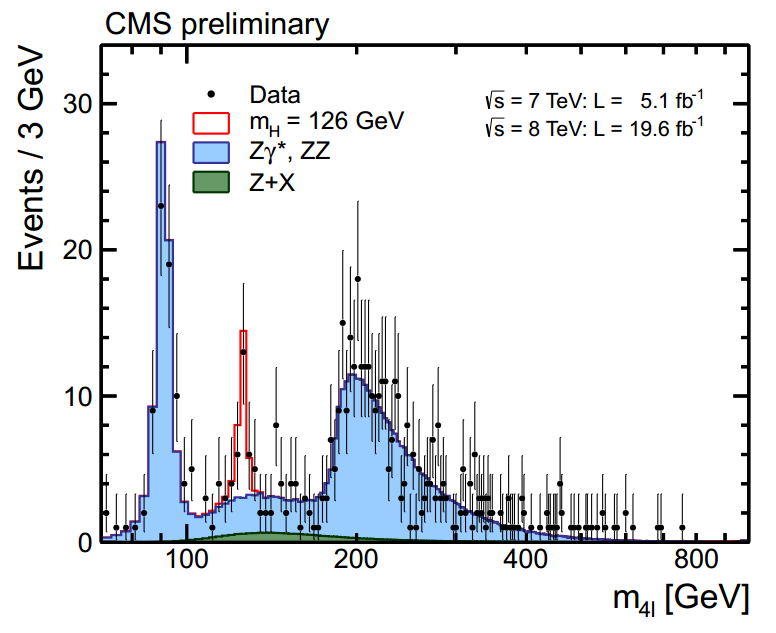
\includegraphics[width=0.45\textwidth]{cms_higgs.png}
    \caption{4-lepton invariant mass showing the background and the Higgs peak.}
\end{figure}

%%%%%%%%%%%%%%%%%%%%%%%%%%%%%%%%%%%%%%%%%%%%%%%%%%%%%%%%%%%%%%%%%%%%%%%%%%%%%%%%
\bibliography{mybibliography}
%%%%%%%%%%%%%%%%%%%%%%%%%%%%%%%%%%%%%%%%%%%%%%%%%%%%%%%%%%%%%%%%%%%%%%%%%%%%%%%%

%%%%%%%%%%%%%%%%%%%%%%%%%%%%%%%%%%%%%%%%%%%%%%%%%%%%%%%%%%%%%%%%%%%%%%%%%%%%%%%%
\end{document}
%%%%%%%%%%%%%%%%%%%%%%%%%%%%%%%%%%%%%%%%%%%%%%%%%%%%%%%%%%%%%%%%%%%%%%%%%%%%%%%%
